\documentclass[sp]{FEIstyle}

% Author of the thesis
\FEIauthor{%
  Bc. Michal Balogh\\
  Bc. Juraj Hušek\\
  Bc. Ján Osadský\\
  Bc. Fridrich Molnár\\
  Bc. Zoltán Renczes
}


% Evidence number
%\FEIregNr{FEI-xxxx-xxxx}

% Title
\FEItitle{Tímový projekt}
\FEItitleEn{Team project}

% Date
\FEIdate{31}{12}{2025}

% Keywords
\FEIkeywords{historické šifry, spracovanie obrazu, digitálna anotácia, kolaboratívna platforma, webová aplikácia}
\FEIkeywordsEn{historical ciphers, image processing, digital annotation, collaborative platform, web application}

% Further details
\FEIstudyProgramme{Aplikovaná informatika}
\FEIstudyProgrammeEn{Applied Informatics}
\FEIstudyField{názov študijného odboru}
\FEIstudyFieldEn{Field of the study in English}
\FEItrainingWorkplace{Názov školiaceho pracoviska}
\FEItrainingWorkplaceEn{Training Work place}
\FEIcourseTag{TP1, TP2}
\FEIcourse{Tímový projekt 1, Tímový projekt 2}
\FEITA{Ing. Stanislav Marochok}
% Supervisor
\FEIsupervisor{tituly Meno Priezvisko, tituly}

% Consultant
% -- if there is none, comment out the next line
\FEIconsultant{tituly Meno Priezvisko, tituly}

% Glossaries -- terms and abbreviations.
% If you use automatic glossaries,
% uncomment the next line.
%\FEIglossaries{includes/glossary}

% Bibliography database file
\bibliography{includes/bibliography.bib}

\begin{document}

%%%%%%%%%%%%%%%%%%
%%              %%
%% FRONT MATTER %%
%%              %%
%%%%%%%%%%%%%%%%%%
\frontmatter

\FEIpdfInfo
\FEIcover
\FEItitlePage
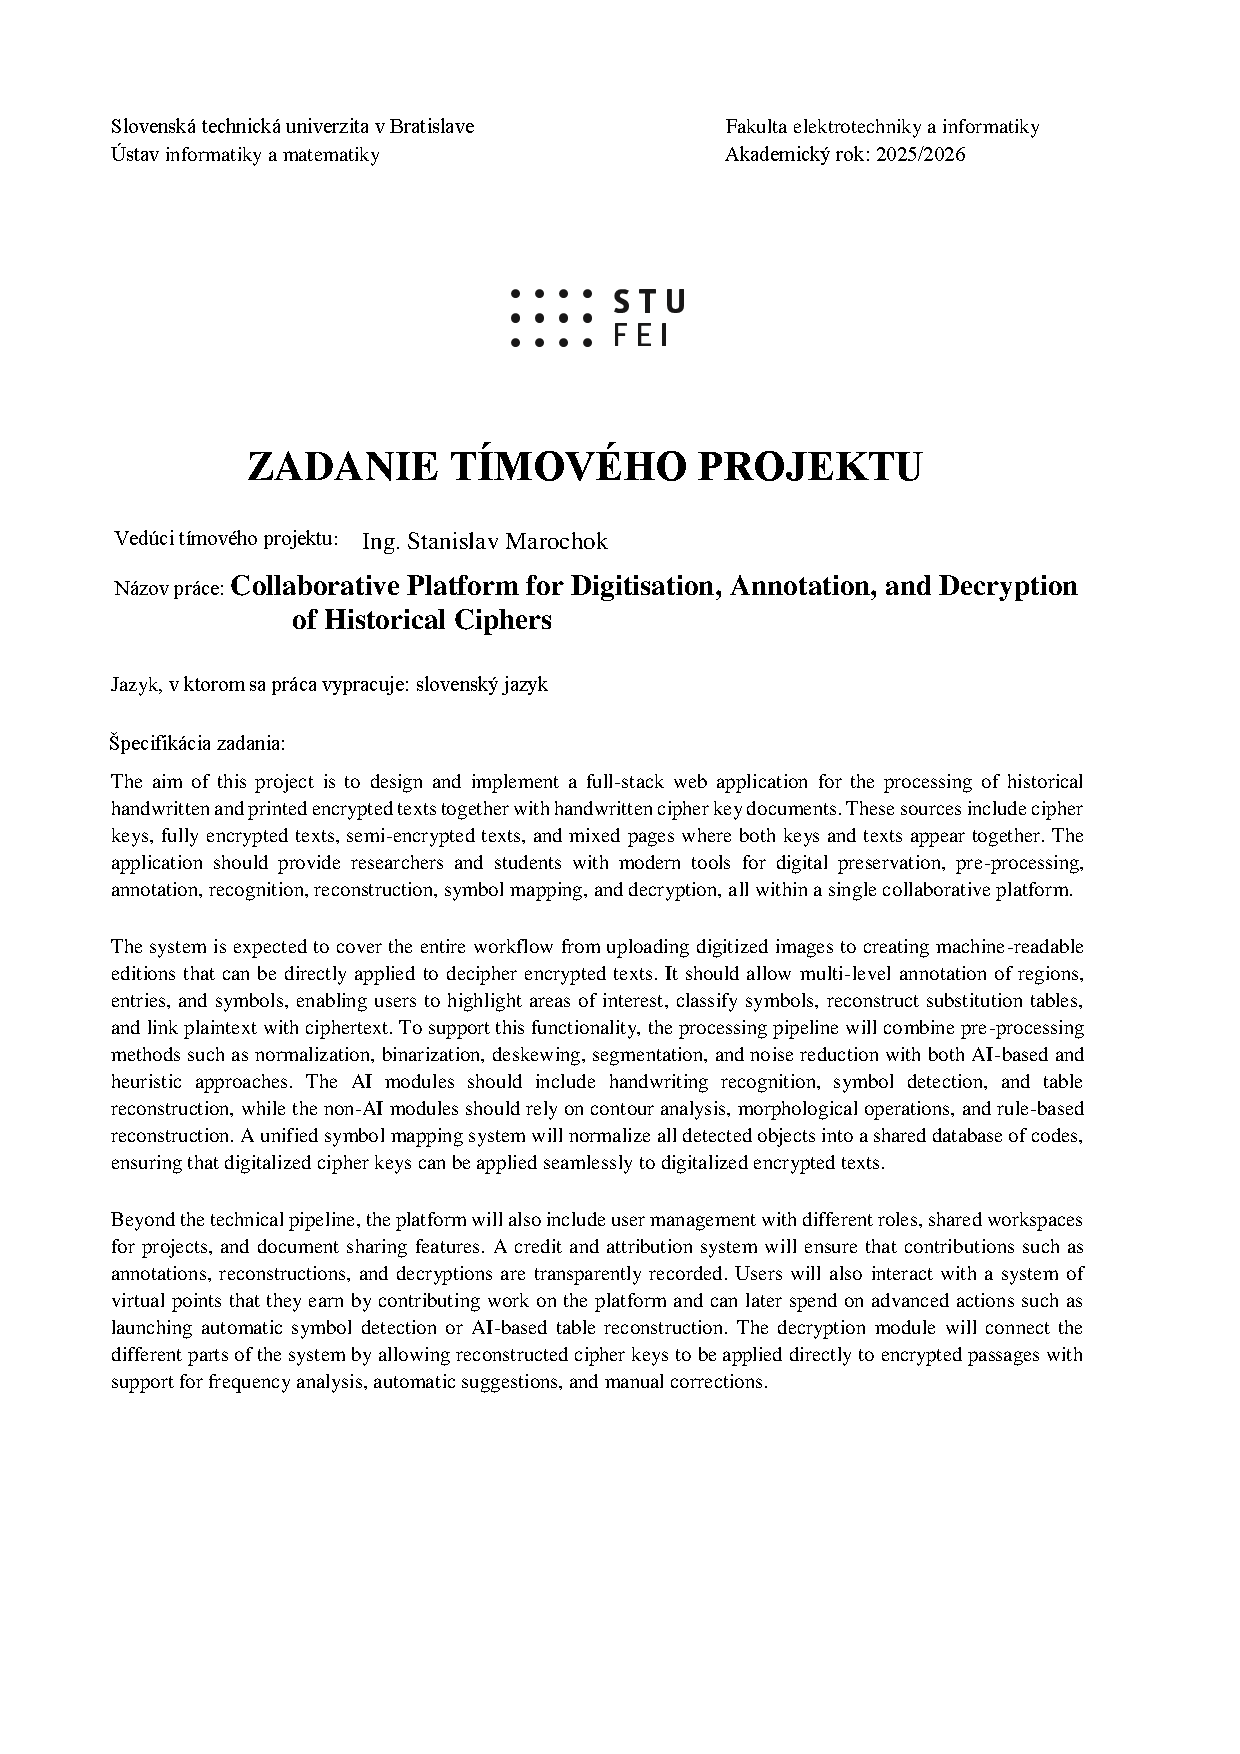
\includepdf[pages=-]{includes/assignment.pdf}
%\FEIthanks{includes/thanks}
\FEIabstract{includes/abstract}
\FEIabstractEn{includes/abstractEN}
\FEIcontent
%\FEIlistOfFiguresAndTables

%% List of units and abbreviations
%%
%% Choose the method of typesetting the list of
%% units and abbreviations.
%% Uncomment only one of the two lines below!

%% METHOD 1:
%% ---------
%% Automatically generated and sorted list of
%% abbreviations with hyperlinks from the text.
%% Edit includes/glossary.tex.
%\FEIlistOfGlossaries
%% METHOD 2:
%% ---------
%% Manual list -- must be manually filled and sorted,
%% does not make hyperlinks from the text.
%% Edit includes/manual_glossary.tex.
\FEImanualListOfGlossaries{includes/manual_glossary}

%% Lists of algorithms and listings
\FEIlistOfAlgorithms
\FEIlistOfListings

%%%%%%%%%%%%%%%%%
%%             %%
%% MAIN MATTER %%
%%             %%
%%%%%%%%%%%%%%%%%
\mainmatter

\FEIintroduction{includes/introduction}
\FEIcore{includes/core}
\FEIconclusion{includes/conclusion}

%% Uncomment only if the document is writen in english
%\FEIresume{includes/resume}

%%%%%%%%%%%%%%%%%%
%%              %%
%% Bibliography %%
%%              %%
%%%%%%%%%%%%%%%%%%
\FEIbibliography
%% AI Declaration
%\FEIaiDeclaration{includes/ai_declaration}

%%%%%%%%%%%%%%%%%%
%%              %%
%% BACK MATTER  %%
%%              %%
%%%%%%%%%%%%%%%%%%
\backmatter

%% Attachment A
%\FEIappendix{Algoritmus\label{att:algorithms}}{includes/attachmentA}

%% Attachment B
%\FEIappendix{Výpis dlhého kódu\label{att:listings}}{includes/attachmentB}

%% Attachment C
%\FEIappendix{Slovníček pojmov\label{att:dictionary}}{includes/attachmentC}

%% Attachement D
%\FEIappendix{Súborová štruktúra projektu\label{att:files}}{includes/attachmentD}


\end{document}
